\FloatBarrier
\section{Registered domain and predictor extensions}
\label{sec:domain-extensions}
The original forecasting gains, mixed planning comparisons, and failed
rollout-context screen remain unchanged. A separately registered 36-run
development campaign has completed training, forecasting and planning on
two additional simulations and a second predictor family. A subsequent
six-run observation-gain ablation is also complete. These adapted tasks
are not reproductions of published drone or surgical leaderboards.
Table~\ref{tab:extension-status} distinguishes completed development
evaluation from final testing, which remains unrun. All positive and
negative outcomes below remain separate from the original test results.

\begin{table}[H]
\centering\small
\setlength{\tabcolsep}{6pt}
\begin{tabular}{p{.42\linewidth}p{.23\linewidth}p{.23\linewidth}}
\toprule
Stage & Drone & Tissue manipulation \\
\midrule
Recorded trajectories & 384 collected & 384 collected \\
Full collection audit & Passed & Passed \\
Reachable-goal protocol & Audited & 112 replay checks passed \\
Frozen visual feature cache & Complete & Complete \\
Full 30-epoch training & 18/18 complete & 18/18 complete \\
Development forecasting & 18/18 complete & 18/18 complete \\
Development planning & 18/18 complete & 18/18 complete \\
Gain ablation: train/forecast/plan & 6/6 in each stage & Not registered \\
Final model test evaluation & Pending & Pending \\
\bottomrule
\end{tabular}
\caption{\textbf{Completed registered extension campaigns.}
Each original domain has two predictor families, three methods and three
training seeds. The subsequent drone ablation has two methods and three
seeds. All models completed 30 epochs and both development evaluations;
pending final tests are unavailable, not zero performance.}
\label{tab:extension-status}
\end{table}

\paragraph{Data and physical tasks.}
Each domain records 384 trajectories of 200 native commands, partitioned into
192 training, 48 validation, 48 development and 96 test trajectories.
Initial-state seed families are disjoint between splits; within a split,
the same seeds are recorded across response gains 1, 0.75 and 1.25.
Five successive two-dimensional commands form one model action block.
Model inputs contain RGB observations and commanded actions. Simulator
state is retained separately for collection verification and scoring.
Action normalization uses only the training split. Photometric transforms
and the seven training/validation appearance--gain combinations follow the
original loader; development uses warm appearance with gain 0.75, while
cool appearance with gain 1.25 is withheld from training.

The drone task adapts \texttt{gym-pybullet-drones}
\citep{panerati2021learning}, pinned at revision \texttt{7ebad1ecabd2}.
A CF2X vehicle receives planar velocity requests through the upstream PID
controller at fixed requested altitude, observed by a fixed external RGB
camera. The intervention scales commanded response; it is not a wind or
mass change. Recorded settled endpoints define goals. Success requires
XY distance below 4\,cm, speed below 6\,cm/s, altitude error below 5\,cm,
and no crash or workspace escape. The complete collection audit checked
all 384 trajectories, payload hashes and 77,184 native states.

The deformable-tissue task adapts LapGym's SOFA tissue manipulation
environment \citep{scheikl2023lapgym}, pinned at revision
\texttt{85bf7e05dd08}. Two-dimensional gripper commands are scaled before
native clipping. Forecast collection and planning-goal verification are
separate: planning goals require an independent recorded-action replay
with the desired marker moved to the recorded endpoint, preserving the
physical trajectory. Native XZ tissue-point distance at most 2\,mm defines
success. All 384 collection episodes passed the full data audit; independent
replays verified all 112 eligible development/test goal references, including
physical-state equality and RGB equality outside the relocated target marker.
Finite workspace-clipped collection transitions are retained;
planning eligibility additionally excludes unstable or invalid reference
trajectories before model evaluation. This is a constrained reachable-goal
distribution, not clinical validation or a claim of autonomous surgical safety.

\paragraph{Predictor families and matched controls.}
Both families reuse the frozen released PushT LeWM visual encoder and its
canonical target coordinates; neither uses drone or surgical visual
pretraining. The first retains the released transformer initialization.
The second replaces its predictor with a two-layer GRU of hidden size 256,
using the same projected state/action interface. The GRU is an in-house
architecture control, not a Dreamer reproduction. Parameter counts and
initialization differ across families; comparisons are primarily within
each family. The three methods are \emph{Framewise calibration},
\emph{ShiftWM (ours)}, and \emph{Constant dynamics context}. The last retains
episode-dependent observation correction but supplies zero inputs to the
dynamics-context network. Its learnable biases permit a nonzero common
response; equal nominal parameter count does not imply equal effective
capacity. Seeds 0, 1 and 2 give 18 runs per domain.

Every run trains for 30 epochs with AdamW, learning rate $10^{-4}$,
cosine minimum $10^{-6}$, weight decay 0.01, gradient clipping 1,
batch size 128 and stride 4. Eight-frame windows provide three observed
support frames and five recursive query targets, including the first
unobserved target. Training uses BF16 where supported; selection uses
the minimum full-validation recursive MSE in float32 (autocast disabled;
CUDA TF32 matrix multiplication remains allowed for every arm). Alignment and context
consistency weights match across the applicable methods. Source, data,
cache, normalization and checkpoint identities are pinned; optimizer and
RNG state support continuation. Training completion alone is not a
planning result or a validated release.

\paragraph{Development planning and decision rule.}
Before model outcomes, select the first eight eligible development
trajectories in seed order at gain 0.75, or report a shortfall if fewer
are available. Initial-goal separation must be at least 8\,cm for the drone
and 4\,mm for tissue manipulation; initially solved tasks are excluded
and every exclusion is retained. Policy-induced invalid actions count
as failures. All methods share goal images, ten recorded support commands,
planner random numbers and a 200-native-command total budget including
support. CEM uses horizon five blocks, 128 candidates, five iterations and
16 elites; it replans after at most five executed commands and retains
the unused plan as its warm start. Search uses standardized action
coordinates, with clipping after conversion to native commands. Report
support-only successes separately and log partial final blocks exactly.

Random actions use the same interaction budget; privileged replay of
recorded actions checks goal reachability. Replay is not a deployable
baseline. We report success counts and rates, paired task and seed
uncertainty, native interactions, physical errors, failures and latency.
Promotion requires better closed-loop success than both
within-family controls with consistent evidence across seeds and domains.
Final test evaluation is separate from development, and any changed
hypothesis or protocol receives a new run namespace. This campaign cannot
turn the original null planning findings into positive evidence by
selectively reporting a favorable domain or model.

\subsection{Completed development comparisons}
\label{sec:drone-development}
All 36 conditions have completed training, forecasting and planning.
Table~\ref{tab:extension-drone} reports every method and training seed for
both domains. No task succeeds during the ten-command common support.
On the drone, transformer ShiftWM achieves 20.83\% success versus
16.67\% for either control; with the GRU it achieves 16.67\%, versus
25.00\% for Framewise and 29.17\% for Constant dynamics.
On tissue manipulation, transformer ShiftWM achieves 4.17\% versus
8.33\% for either control, while GRU ShiftWM achieves 12.50\% versus
8.33\% for either control. These opposite signs across families and
domains do not establish a general benefit of inferred dynamics context.

Table~\ref{tab:extension-paired} retains the matched task structure when
quantifying uncertainty: it jointly resamples training seeds and physical
task seeds in 5,000 crossed bootstrap draws. No original interval has a
strictly positive lower bound. Forecast MSE and planning success need not
agree: drone GRU ShiftWM has lower horizon-five error than either control
but lower closed-loop success. Final test results are not used here, and
these development results do not satisfy the promotion rule above.

The fixed random-action control succeeds on 2/8 drone and 1/8 tissue tasks;
privileged recorded-action replay succeeds on 8/8 in each domain.
Random uses base seed 101 plus each task seed, with no independently
trained models; replay is a reachability check. Original drone ShiftWM
in both predictor families is below the random 25\% point estimate.
Neither this drone task nor the tissue simulation establishes useful
real-world control or clinical performance.

\begin{table}[H]
\centering\small
\setlength{\tabcolsep}{4pt}
\begin{tabular}{lrrrrr}
\toprule
Method & Seed 0 & Seed 1 & Seed 2 & Success (\%) & MSE@5 ($10^{-3}$) \\
\midrule
\multicolumn{6}{l}{\emph{Drone / Transformer}} \\
Framewise & 1/8 & 2/8 & 1/8 & 16.67 & 5.650 \\
Constant dynamics & 1/8 & 1/8 & 2/8 & 16.67 & 5.718 \\
ShiftWM (ours) & 1/8 & 2/8 & 2/8 & 20.83 & 5.711 \\
\addlinespace[3pt]
\multicolumn{6}{l}{\emph{Drone / GRU}} \\
Framewise & 1/8 & 3/8 & 2/8 & 25.00 & 6.578 \\
Constant dynamics & 1/8 & 4/8 & 2/8 & 29.17 & 6.591 \\
ShiftWM (ours) & 1/8 & 2/8 & 1/8 & 16.67 & 6.503 \\
\addlinespace[3pt]
\multicolumn{6}{l}{\emph{Tissue manipulation / Transformer}} \\
Framewise & 0/8 & 1/8 & 1/8 & 8.33 & 3.588 \\
Constant dynamics & 1/8 & 1/8 & 0/8 & 8.33 & 3.563 \\
ShiftWM (ours) & 1/8 & 0/8 & 0/8 & 4.17 & 3.573 \\
\addlinespace[3pt]
\multicolumn{6}{l}{\emph{Tissue manipulation / GRU}} \\
Framewise & 0/8 & 1/8 & 1/8 & 8.33 & 4.405 \\
Constant dynamics & 0/8 & 1/8 & 1/8 & 8.33 & 4.417 \\
ShiftWM (ours) & 0/8 & 1/8 & 2/8 & 12.50 & 4.389 \\
\addlinespace[3pt]
\bottomrule
\end{tabular}

\caption{\textbf{Complete development comparison, all 36 original models.}
Within each domain, each seed uses the same eight planning tasks and a
200-native-command budget including support. Success is the mean over
three training seeds; the 24 seed--task instances are not 24 independent
physical tasks. MSE@5 is mean fixed-reference forecasting error across
the three seeds, on identical development windows (lower is better).
All controls are matched in-house implementations within each family.}
\label{tab:extension-drone}
\end{table}

\begin{table}[H]
\centering\small
\setlength{\tabcolsep}{4pt}
\begin{tabular}{lllrr}
\toprule
Domain & Predictor & Comparator & $\Delta$ (pp) & Paired 95\% interval (pp) \\
\midrule
Drone & Transformer & Framewise & \positivegain{+4.17} & $[-25.00, +33.44]$ \\
Drone & Transformer & Constant dynamics & \positivegain{+4.17} & $[-25.00, +33.33]$ \\
Drone & GRU & Framewise & -8.33 & $[-29.17, +12.50]$ \\
Drone & GRU & Constant dynamics & -12.50 & $[-37.50, +12.50]$ \\
Tissue & Transformer & Framewise & -4.17 & $[-25.00, +12.50]$ \\
Tissue & Transformer & Constant dynamics & -4.17 & $[-20.83, +0.00]$ \\
Tissue & GRU & Framewise & \positivegain{+4.17} & $[+0.00, +25.00]$ \\
Tissue & GRU & Constant dynamics & \positivegain{+4.17} & $[+0.00, +25.00]$ \\
\bottomrule
\end{tabular}

\caption{\textbf{ShiftWM (ours) minus matched controls in planning success.}
Differences are percentage points. \positivegain{Bold green} marks
positive point differences, not statistical significance. Intervals use
paired crossed resampling of three training and eight physical task
seeds; they are unadjusted exploratory 95\% intervals. All intervals
include or touch zero, and all negative comparisons remain visible.}
\label{tab:extension-paired}
\end{table}

\subsection{Goal geometry and controlled action-ranking diagnostics}
\label{sec:extension-diagnostics}
The following diagnostics use only training/development evidence and were
motivated by the unsuccessful planning comparisons. They distinguish a
representational limitation from an identified cause of failure.

\paragraph{A fixed-context capacity bound.}
Across all sixteen gain-0.75 development endpoint goals (120 pairs),
the warm appearance transform reduces mean pairwise latent MSE to
17.4\% of the canonical value. In Figure~\ref{fig:goal-geometry}, the
transformer seed-0 Framewise and ShiftWM corrections retain 17.0\% and
16.2\%, respectively. For each observation context, all goals receive
the same correction; measurements are then averaged over sixteen contexts.
If $G(u,c)=g(c)\odot u+b(c)$ and each coordinate of $g(c)$ lies in
$[0.9,1.1]$, its shared translation cancels and
\begin{equation}
0.81\lVert u-v\rVert_2^2
\;\leq\;\lVert G(u,c)-G(v,c)\rVert_2^2
\;\leq\;1.21\lVert u-v\rVert_2^2.
\label{eq:fixed-context-geometry}
\end{equation}
Thus the existing observation FiLM can expand this warm-goal mean separation
to at most 21.1\% of its canonical value in the fixed-context comparison.
This is a capacity bound on pairwise separation, not an achieved result,
an uncertainty interval, or a proof that larger distances improve control.
Framewise calibration lacks this FiLM bound but also fails to recover
canonical separation in this diagnostic. Canonical features themselves
only imperfectly order physical distance, which is only one component
of the drone success criterion.

\begin{figure}[H]
\centering
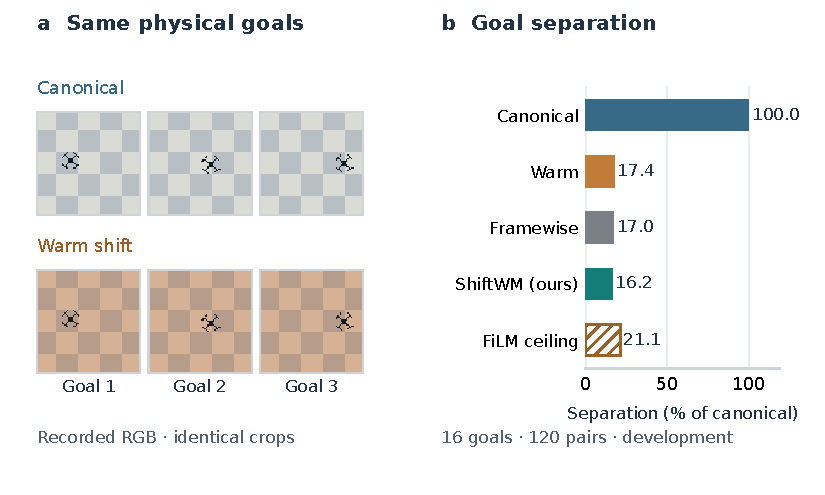
\includegraphics[width=\linewidth]{figures/goal_geometry.pdf}
\caption{\textbf{Development goal geometry under the appearance shift.}
Left: three recorded drone goals selected by minimum, median and maximum
X position, shown with identical central $80\!\times\!80$ crops and the
registered warm transform. Right: mean pairwise latent MSE for all
sixteen goals, normalized by canonical separation; correction uses fixed
support contexts and transformer seed 0. The hatched bar is the analytic
$1.21\times$ expansion ceiling for original observation FiLM applied to
warm features. It is not a new-method measurement or a causal explanation
of planning failure.}
\label{fig:goal-geometry}
\end{figure}

\paragraph{Four-state counterfactual action probe.}
Six seed-0 models score the same fixed library of 32 candidate sequences
from each of four development support states before any candidate is
executed. Each of the 128 branches independently resets and exactly
replays the ten-command support, then executes up to 25 future commands.
Two branches reach a workspace boundary before the full horizon; all
branches are retained, while equal-horizon, safe branches define the
within-task rank correlations and regret. All 24 model-selected winners
are safe. This probe uses actual alternative action executions from a
common state, not merely same-seed trajectories collected under different
response gains: the latter use state-dependent feedback and do not have
identical action histories.

Realized latent cost compares the canonical encoding of each executed
future image with that model's adapted goal; these future images are used
only for the post-execution audit. For transformer ShiftWM, mean Spearman
correlation between predicted and realized latent goal costs is 0.422;
for GRU ShiftWM it is 0.278.
Correlations are computed within each task and then averaged over the
four tasks. Realized latent-cost versus physical-distance correlations
are approximately 0.675, compared with 0.814 using frozen canonical
feature-to-goal costs. The transformer ShiftWM and Constant dynamics
models choose the same candidate on all four tasks, with mean terminal
distance 61.7\,mm and regret 40.9\,mm relative to the best safe candidate.
Transformer Framewise gives 66.4\,mm and 45.6\,mm; all three GRU variants
choose the same candidates, giving 157.5\,mm and 136.6\,mm. The 177.4\,mm
uniform mean over the candidate library is a descriptive reference,
not the random closed-loop controller. These $n=4$ observations suggest
both imperfect action-conditioned ranking and imperfect goal geometry;
they neither isolate a unique mechanism nor establish performance on a
larger task population. In particular, identical selected actions for
inferred and constant contexts do not demonstrate a dynamics-inference
benefit.

\paragraph{Completed, separately registered capacity ablation.}
The six-run transformer study changes only the observation gain to
$g(s)=\exp\{\log(4)\tanh[0.1s/\log(4)]\}$, comparing inferred and constant
dynamics context at seeds 0, 1 and 2. The attainable gain range becomes
$[0.25,4]$, while identity initialization, derivative 0.1 at zero,
parameter shapes, translation, action modulation, losses and the complete
30-epoch training schedule remain matched. Higher-order curvature also
changes, so optimization trajectories need not match. This is a
capacity ablation, not a claim of algorithmic novelty. Its versioned
checkpoints and output namespace are separate from the original study.

All six runs completed 30 epochs and both development evaluations
(Table~\ref{tab:extension-geometry}). Revised ShiftWM reaches 7/24
task--seed instances, versus 4/24 for the revised Constant dynamics
control: $+12.50$ percentage points, with a paired exploratory interval
$[0,37.50]$. Each training seed gains one of eight successes, with three
ShiftWM-only successes and no control-only success across the matched
instances. Relative to original ShiftWM (5/24), there are three new
successes and one lost success. The difference is $+8.33$ points,
with interval $[-12.50,29.17]$. The revised Constant dynamics control retains 4/24 in aggregate
but changes which tasks succeed. The revised ShiftWM rate, 29.17\%,
exceeds the single random-policy reference of 25\% only descriptively.

These are subsequent comparisons on the same development tasks. The
forecast MSE changes little, and the fixed 16-goal/120-pair geometry
measurement has not yet been repeated for the revised checkpoints.
Consequently, the observed success increases do not demonstrate restored
goal geometry, improved action ranking, or independent generalization.
They do not justify promoting the method to final-test evaluation.

\begin{table}[H]
\centering\small
\setlength{\tabcolsep}{4pt}
\begin{tabular}{lrrrrr}
\toprule
Method & Seed 0 & Seed 1 & Seed 2 & Success (\%) & MSE@5 ($10^{-3}$) \\
\midrule
\multicolumn{6}{l}{\emph{Original narrow gain}} \\
Constant dynamics & 1/8 & 1/8 & 2/8 & 16.67 & 5.718 \\
ShiftWM (ours) & 1/8 & 2/8 & 2/8 & 20.83 & 5.711 \\
\addlinespace[3pt]
\multicolumn{6}{l}{\emph{Revised wide gain}} \\
Constant dynamics & 0/8 & 2/8 & 2/8 & 16.67 & 5.724 \\
ShiftWM (ours) & 1/8 & 3/8 & 3/8 & 29.17 & 5.713 \\
\addlinespace[3pt]
\bottomrule
\end{tabular}
\par\vspace{5pt}
\begin{tabular}{lrr}
\toprule
Paired contrast & $\Delta$ (pp) & Paired 95\% interval (pp) \\
\midrule
Wide ShiftWM (ours) $-$ wide constant & \positivegain{+12.50} & $[+0.00, +37.50]$ \\
Wide ShiftWM (ours) $-$ original ShiftWM (ours) & \positivegain{+8.33} & $[-12.50, +29.17]$ \\
Wide constant $-$ original constant & +0.00 & $[-25.00, +33.33]$ \\
\bottomrule
\end{tabular}

\caption{\textbf{Completed observation-gain ablation on drone development.}
Original and revised transformer conditions share data, optimization,
validation selection, eight physical tasks, support and planner budget.
The six revised models use seeds 0, 1 and 2. The lower panel reports
paired crossed-bootstrap success differences; all intervals include or
touch zero. \positivegain{Bold green} marks positive point estimates
only. This follow-up ablation is exploratory, not an independent test
of the geometry hypothesis.}
\label{tab:extension-geometry}
\end{table}

\subsection{Separate official AdaJEPA reproduction}
\label{sec:official-adajepa}
We additionally ran the released AdaJEPA implementation
\citep{wang2026adajepa}, pinned at revision \texttt{51d8665b7978}, with
its official PushT checkpoint and evaluation goals. All four 50-episode
evaluations completed (Table~\ref{tab:official-adajepa}). The model
observes RGB plus agent proprioception; the released goals, pretrained
representation and planner budget differ from our RGB-only studies.
These results therefore remain a separate reproduction, without a
direct performance ranking against ShiftWM.

Official CEM uses horizon 25, 200 candidates, 30 elites and ten
optimization iterations, with at most 20 replans and five grouped
actions executed per replan (frameskip five). All stages use evaluation
seed 100. Adaptive success exceeds frozen success by 24 percentage
points on clean observations and 20 under blur. Aggregate logs and one
evaluation seed do not support a paired task-level uncertainty interval.
This is evidence that the released adaptive implementation runs locally
under its own protocol, not a state-of-the-art or matched-baseline claim.

The checkpoint, goals, official configuration and scientific command
are pinned for every stage. The first clean-frozen run began before
launcher/runtime hashes were added to the record; a supplemental GPU
observation documents its hardware. Later stages include those metadata
fields, but current hashes cannot retroactively establish their exact
values at the first stage's launch.

\begin{table}[H]
\centering\small
\setlength{\tabcolsep}{7pt}
\begin{tabular}{lrrr}
\toprule
Observation & Official frozen & Official adaptive & $\Delta$ (pp) \\
\midrule
Clean & 34/50 (68\%) & 46/50 (92\%) & \positivegain{+24.00} \\
Blur & 29/50 (58\%) & 39/50 (78\%) & \positivegain{+20.00} \\
\bottomrule
\end{tabular}

\caption{\textbf{Official AdaJEPA reproduction under its separate protocol.}
Each entry uses 50 released evaluation goals and seed 100, with RGB plus
agent proprioception. Differences compare adaptive and frozen execution
within this official protocol. \positivegain{Bold green} marks positive
aggregate point differences; no paired interval or significance claim
is made. These inputs and budgets are not matched to ShiftWM.}
\label{tab:official-adajepa}
\end{table}
